
\chapter{Energy and Institution Size}
\label{Ch_energy}

\section*{Abstract}
Why do institutions grow? Despite nearly a century of scientific effort, there remains little consensus on this topic. This paper offers a new approach that focuses on energy consumption. A systematic relation exists between institution size and energy consumption per capita: as energy consumption increases, institutions become larger. I hypothesize that this relation results from the interplay between technological complexity and human biological limitations. I also show how a simple stochastic model can be used to link energy consumption with firm dynamics.



\section{Introduction}

Throughout the last century, there has been a recurrent desire to connect human social evolution to changes in energy consumption \cite{cottrell_energy_2009,hall_hydrocarbons_2003,soddy_virtual_1926,white_energy_1943}. The motivation is simple: the laws of thermodynamics dictate that any system that exists far from  equilibrium must be supported by a flow of energy \cite{kondepudi_modern_1998}.  Since human societies are non-equilibrium systems, it follows that energy flows ought play an important part in social evolution. However, it has proved difficult to move from grand pronouncements based on the laws of thermodynamics to a \emph{quantitative} understanding of the relation between energy use and social evolution \cite{adams_man_1978}. This paper offers a contribution to such a quantitative understanding.

This paper is concerned with one particular aspect of social change: the growth in size of the \textit{institutions that control human labor}. While such institutions have taken many forms throughout history, in the modern era, the control of human labor is dominated by two institutions: the \textit{business firm} and \textit{government}. In this paper, institution \textit{size} refers to the amount of human labor (i.e employment) controlled by an organization. Under this definition/metric of institution size, I demonstrate that a  pervasive, positive correlation exists between institution size and energy use per capita. 


I pursue  two avenues for understanding the relation between energy and institution size. The first approach draws on the rich history of stochastic  modelling within firm size theory. Stochastic (random) models have been successfully used to link firm \emph{dynamics} to the overall firm size distribution. Yet there is little understanding of what drives variations in firm dynamics. Using data on firm age and firm size to constrain a stochastic model, I demonstrate that firm dynamics are likely related to rates of energy consumption, and I offer a prediction of what this relation should look like.


The second approach is more speculative, and aims to offer a general explanation of why rates of energy consumption are related to institution size. I propose two factors that mediate this relation: \textit{technological scale} and \textit{social hierarchy}. I hypothesize that increases in energy consumption involve a trend towards the use of technologies that are larger and more complex. These increasingly large technologies require the coordination of greater numbers of people. Given the limitations of the human brain \cite{dunbar_neocortex_1992}, I argue that large-scale social coordination is most easily achieved through social \textit{hierarchy} \cite{turchin_evolution_2009} and that firms and government are specific manifestations of this hierarchy. 



\section{Theories of Institutional Size}
\label{Sec_literature}

Theories of institution size can be divided into two classes: those that concern themselves with the \emph{causes} of institutional growth (`why' theories) and those that do not (`how' theories). `How' theories have met with great empirical success, while `why' theories have struggled to offer explanations that are testable.

All `how' theories  of institutional size can be traced back to the work of the French economist Robert Gibrat, who discovered that the rate of growth of business firms seemed to be \emph{independent} of their size \cite{gibrat_les_1931}. While later investigation  found this `law of proportional effect' to be only approximately true --- growth rate variance tends to decline with size  \cite{hart_size_1962,hymer_firm_1962,singh_size_1975} ---  it has led to a rich history of stochastic firm growth models \cite{de_wit_firm_2005,sutton_gibrats_1997}. The basic principle is that firm growth is treated probabilistically. Each firm is submitted to a series of random shocks that make it grow (or shrink) over time. When applied to large numbers of firms, the result is a firm size \emph{distribution}. The surprising finding is that these purely random models can very accurately predict the functional form of real-world  firm size distributions. 

Despite their success, `how' theories are not particularly satisfying because they do not explain \emph{why} institutions grow. Unfortunately, theories that \emph{do} attempt to explain the cause of institution growth often rely on unmeasurable variables, and as a result, are untestable.

The theory of the firm has been dominated by Ronald Coase's  \textit{transaction cost} approach. According to Coase, ``... a firm will tend to expand until the costs of organizing an extra transaction within the firm become equal to the costs of carrying out the same transaction by means of an exchange on the open market or the costs of organizing in another firm'' \cite{coase_nature_1937}. Unfortunately, transaction costs have been notoriously difficult to define (let alone measure), rendering Coasian theory  untestable  \cite{geroski_growth_1999,nitzan_capital_2009}

Other theories propose that management talent is the driver of firm growth.  For instance, Robert Lucas assumes that the firm size distribution results from ``allocat(ing) productive factors over managers of different ability so as to maximize output'' \cite{lucas_jr_size_1978}. Yet Lucas concedes that the causal factor in this model --- the talent of managers --- is  ``probably unobservable''. Despite this problem, Lucas's theory remains popular \cite{gomes_human_2014,poschke_firm_2014}.

Still other theories propose that firm growth is the result of a resource-driven competitive advantage \cite{barney_firm_1991,peteraf_cornerstones_1993}. Unfortunately, this approach has struggled to stipulate exactly how a particular resource is transformed into a value-creating competitive advantage. Priem and Butler argue that the `resource-based view' advances a theory of value that is tautological --- resources create \emph{value} because they are (among other things) \emph{valuable} \cite{priem_tautology_2001}. 

In terms of measurability, theories of government size have faired no better than theories of firm size. One approach is to apply the rational-choice model to the behavior of voters. Government size is treated as a reflection of the preferences of utility maximizing voters \cite{meltzer_rational_1981,peltzman_growth_1980}.
However, without an objective measure of individuals' internal preferences, this theory is untestable.

Another approach is to assume that government bureaucracies (or government as a whole) are self-serving entities that attempt to maximize their budgets, but are restrained by voters and/or an institutional framework such as the constitution 
\cite{brennan_power_1980,niskanen_bureaucracy_1974}.   While maximizing behavior is one of the fundamental postulates of neoclassical economics, the hypothesis that humans maximize external pay-offs has been falsified \cite{henrich_search_2001}. 

The lack of measurable variables has consistently plagued `why' theories of institution size. If a new theory is to be successful, it must demonstrate a connection between institution size and some universally measurable quantity. Energy consumption is just such a quantity. 




\section{Energy and Institution Size: Empirical Evidence}
\label{Sec_Evidence}



To study the relation between energy and institution size, I compare variations in energy use per capita  to variations in the size of firms and government over both space and time. For firms, I investigate how changes in the  base, tail and mean of the firm size distribution are related to changes in energy use per capita. I use self-employment data to investigate the base of the firm size distribution (relying on the assumption that self-employer firms are very small). To investigate the tail of the firm size distribution, I look at the employment share of the largest firms. To quantify the relative size of government, I measure the government share of total employment.





%%%%%%%%%%%%%%%%%%%%%%%%%%%%%%%%%%%%%%%%%%%%%%%%%%%%%%%%%%%5
\begin{figure}
	
	\centerline{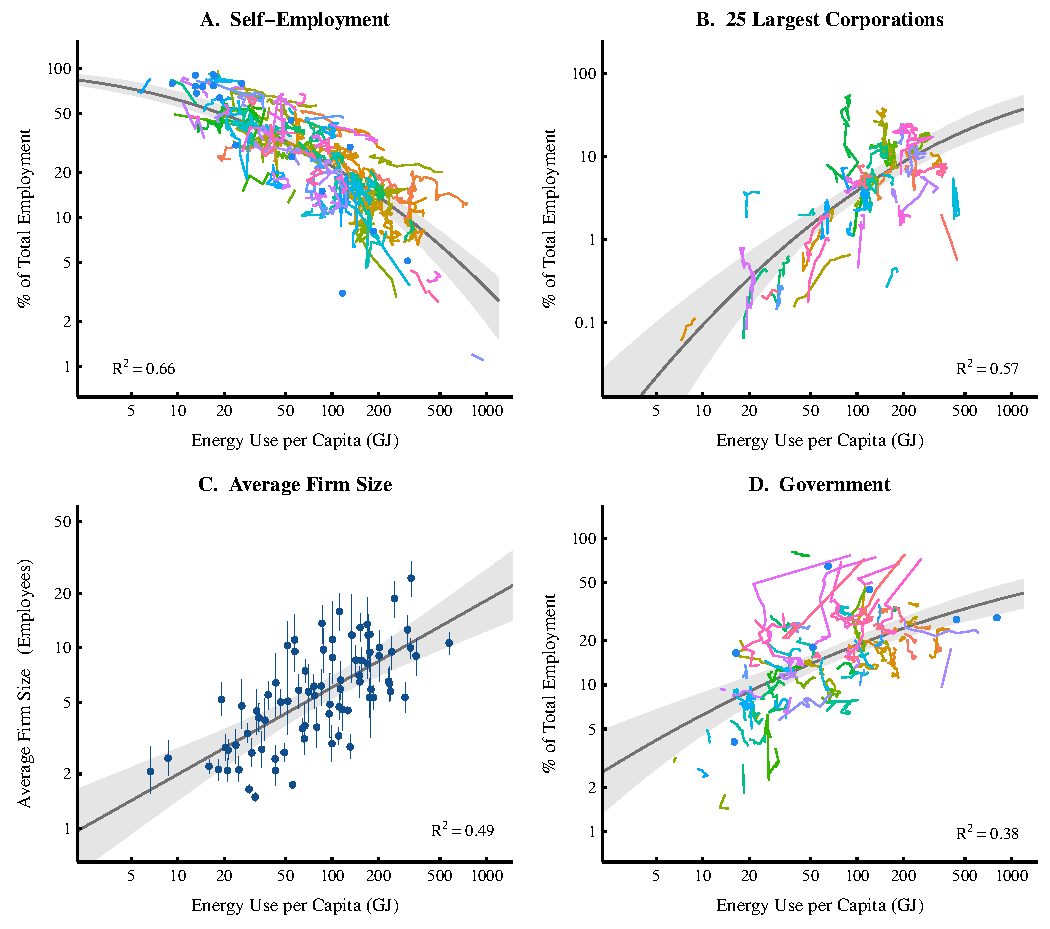
\includegraphics[scale=1]{Fig1}}
	
	\caption{Institution Size vs. Energy Use per Capita at the International Level\label{Fig_Global_inst}}
	
	\small
	\smallskip
	
	
	This figure shows how different metrics of institution size vary with energy consumption per capita. Panels A-C analyze variations in firm size by looking at the base, tail, and estimated mean of the firm size distribution. Panel D analyzes variations in government size. In order to show as much evidence as possible, panels A, B and D are a mix of time series and scatter plot. Lines represent the path through time of individual countries while points represent a country with a single observation.  Error bars in panel C represent the 95\% confidence interval of mean firm size estimates.  Variations in self-employment, large-firm, and government employment share vs. energy are modelled with log-normal cumulative distribution functions. Mean firm size vs. energy is modelled with a power law. Grey regions indicate the 99\% confidence region of each model. For sources and methodology, see Appendix \ref{App_sources}.
	
\end{figure}

\begin{figure}
	
	\centerline{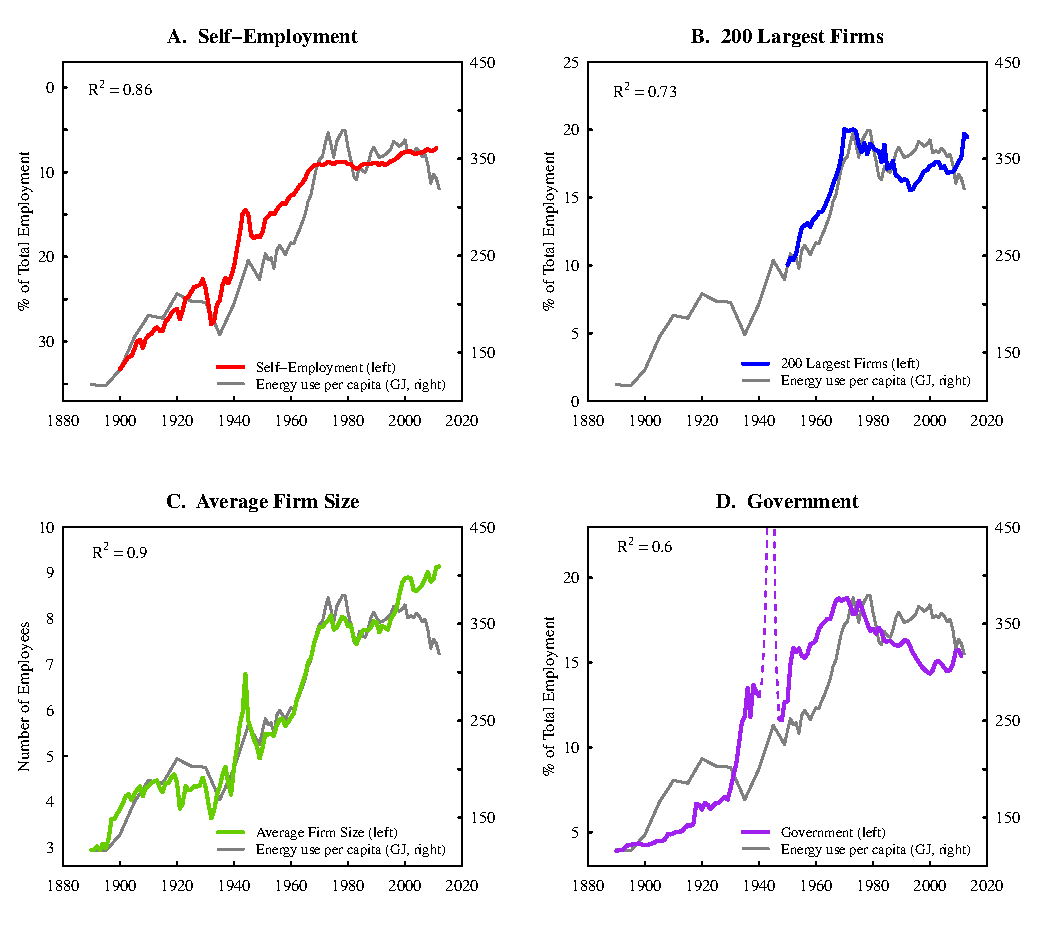
\includegraphics[scale=1]{Fig2}}
	
	\caption{Institution Size vs. Energy Use per Capita in the United  States\label{Fig_US_inst}}
	
	\small
	\smallskip
	
	This figure shows the trends for various measures of institution size in the United States over the last century. Trends mirror those found at the global level. As energy consumption per capita increases, self-employment rates decline (panel A, note reverse scale), the large firm employment share increases (panel B), mean firm size increases (panel C), and the government employment share increases (panel D). Note that government regressions exclude World War II (dotted line). For sources and methodology, see Appendix \ref{App_sources}.
	
	\bigskip
	
\end{figure}


\begin{figure}
	
	\centerline{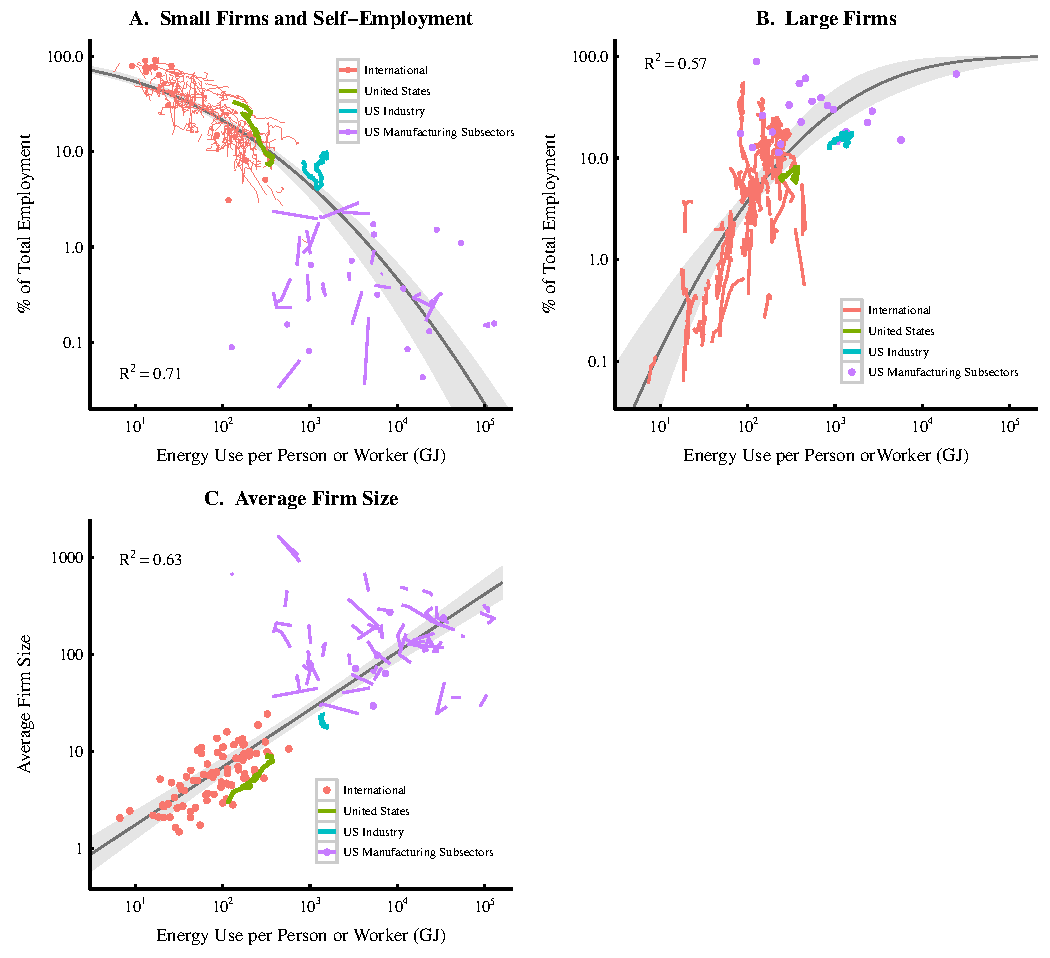
\includegraphics[scale=1]{Fig3}}
	
	\caption{Synthesizing Evidence --- Firm Size vs. Energy Use per Person or Worker\label{Fig_E_Aggregate}}
	
	\small
	\smallskip
	
	This figure combines data from 3 different units of analysis (nations, sectors, and sub-sectors) to offer a comprehensive picture of the relation between firm size and energy use per capita (or per worker). `US Industry' consists of construction and manufacturing sectors, while  `US Manufacturing Subsectors' are the smallest subdivisions of the manufacturing sector. At the national level, energy use is measured per \textit{person}, while at the sectoral level, it is measured per \textit{worker}. In panel A, self-employment data (for nations and US Industry) is merged with the data for the employment share of firms with 0-4 employees in US manufacturing subsectors. In panel B, data for the employment share of the largest 25 firms (for nations and US Industry) is merged with data for the employment share of firms with more than 5000 employees in US manufacturing subsectors. Panel C shows mean firm size data at the national and sectoral level.  Grey regions indicate the 99\% confidence region of each model. For sources and methodology, see Appendix \ref{App_sources}.
	
\end{figure}
%%%%%%%%%%%%%%%%%%%%%%%%%%%%%%%%%%%%%%%%%%%%%%%%%%%%




Comparison of these institution size metrics with energy use per capita are shown in Figures \ref{Fig_Global_inst}-\ref{Fig_E_Aggregate}. Figure \ref{Fig_Global_inst} shows international trends (each colored line represents the path through time of a specific country), while Figure \ref{Fig_US_inst} shows time-series data for United States. Figure \ref{Fig_E_Aggregate} (which focuses only on firms) merges data from Figures \ref{Fig_Global_inst}-\ref{Fig_US_inst} and adds US \emph{sectoral} and \emph{subsectoral} level data. Although this synthesis merges data that are not identically defined (see Fig. \ref{Fig_E_Aggregate} caption), the result is clear: the inclusion of sectoral data serves to extend (by two orders of magnitude) the  trends found at the national level. In the case of small firms and mean firm size, the inclusion of sectoral data also increases the regression strength.


To summarize our findings, the evidence in Figures \ref{Fig_Global_inst}-\ref{Fig_E_Aggregate} suggests the following `stylized' facts. As energy use per capita increases:


\begin{enumerate}[noitemsep]
	\leftskip 3em
	
	\item The small firm employment share \emph{declines};
	\item The large firm employment share \emph{increases};
	\item The mean firm size \emph{increases};
	\item The government employment share \emph{increases}.
	
\end{enumerate}

Findings 1-3 suggest that increases in energy consumption are associated with a shift in employment from small to large firms. This indicates that the firm size distribution becomes more \emph{skewed} as energy consumption increases. In the Appendix, I demonstrate that this shift (at the national level) can be accurately modelled in terms of the changing exponent of a power law distribution.

Assuming a correlation between energy use and GDP, then the evidence presented here is consistent with previous research that has focused on the relation between firm size and GDP per capita  \cite{beck_financial_2003,biggs_what_1986,gollin_nobodys_2008,lucas_jr_size_1978,poschke_firm_2014}.
However, my focus here on energy use (rather than GDP) is intentional: it is part of a larger effort to ground economic theory in the laws of thermodynamics \cite{georgescu-roegen_entropy_1971}, and to root empirical analysis in  biophysical (rather than monetary) phenomena \cite{ayres_exergy_2003,cleveland_energy_1984,fix_rethinking_2015,hall_energy_2012}.

Following the long-standing division in institution size theory between `how' and `why' theories, I adopt two separate approaches for understanding the relation between institution size and energy consumption. The first approach deals with the `how' question: \emph{how} exactly do changes in firm size occur? To answer this question, I use a stochastic model to illuminate the relation between energy use and firm dynamics. The second approach deals with the more difficult `why' question: \emph{why} is institution size related to energy consumption. To answer this question, I investigate the relation between energy, technological change, and social coordination.














